\chapter{Integrales y excedentes económicos}
\label{cap:integrales}

\section{La operación inversa de la derivada}

Si la derivada \emph{desarma} un total en su ritmo de cambio (del costo total al costo marginal), la \textbf{integral} hace lo contrario: \emph{rearma} el total a partir del ritmo de cambio. Conocido el costo marginal, integrando recuperamos el costo total; conocido el ingreso marginal, recuperamos el ingreso. Esta dualidad —el Teorema Fundamental del Cálculo— es la que nos permitirá medir áreas con significado económico \cite{chiang}.

\begin{definicion}[Integral definida]
La \emph{integral definida} de una función $f$ entre $a$ y $b$ es el área (con signo) bajo la curva $f$ en ese intervalo:
\[
\int_a^b f(x)\dd x .
\]
Si $F$ es una primitiva de $f$ (es decir, $F'=f$), entonces $\displaystyle\int_a^b f(x)\dd x = F(b)-F(a)$.
\end{definicion}

\section{Recuperar totales a partir de marginales}

Como el costo marginal es la derivada del costo total, integrarlo lo reconstruye:
\begin{equation}
C(q) = \int_0^q \cmg(u)\dd u + CF.
\label{eq:costo_desde_cmg}
\end{equation}
Acá aparece un detalle conceptual importante y fuente de errores frecuentes: \textbf{la integral recupera la parte variable, pero no el costo fijo}. La integración deja indeterminada una constante, y esa constante es justamente el costo fijo $CF$, que hay que sumar aparte porque no proviene de producir unidades. Para el ingreso, en cambio, la condición natural $I(0)=0$ (no vender no genera ingreso) fija la constante en cero.

\begin{ejemplo}[Del costo marginal al costo total]
Si $\cmg(q) = 10 + q$ y el costo fijo es $CF=50$, entonces
\[
C(q) = \int_0^q (10+u)\dd u + 50 = \Big[10u + \tfrac{u^2}{2}\Big]_0^q + 50 = 10q + \tfrac{q^2}{2} + 50,
\]
que es exactamente la función de costo total del Ejemplo del Capítulo~\ref{cap:marginal}. La derivada y la integral son, en efecto, caminos de ida y vuelta.
\end{ejemplo}

\section{El excedente del consumidor}

Acá la integral despliega todo su valor económico. Recordemos la demanda inversa $p(Q)$: indica el \emph{máximo} precio que alguien está dispuesto a pagar por cada unidad. Las primeras unidades se valoran mucho (precio de reserva alto); las últimas, menos. Pero en el mercado \emph{todas} se pagan al mismo precio de equilibrio $p^{*}$. La diferencia entre lo que la gente \emph{estaba dispuesta a pagar} y lo que \emph{efectivamente pagó} es una ganancia neta de bienestar para los consumidores.

\begin{definicion}[Excedente del consumidor]
Es el área entre la curva de demanda inversa y el precio de equilibrio, entre $0$ y la cantidad de equilibrio:
\[
EC = \int_0^{q^{*}} \big(p_d(Q) - p^{*}\big)\dd Q .
\]
\end{definicion}

\section{El excedente del productor}

Simétricamente, la oferta inversa $p_s(Q)$ indica el \emph{mínimo} precio al que los productores aceptan vender cada unidad (su costo marginal). Si el precio de mercado supera ese mínimo, el productor gana la diferencia.

\begin{definicion}[Excedente del productor]
Es el área entre el precio de equilibrio y la curva de oferta inversa:
\[
EP = \int_0^{q^{*}} \big(p^{*} - p_s(Q)\big)\dd Q .
\]
\end{definicion}

La suma $EC + EP$ es el \textbf{excedente total} o bienestar que el mercado genera. Aquí conviene una advertencia que el curso remarca: integrar directamente la diferencia entre demanda y oferta, $\int_0^{q^{*}}(p_d - p_s)\dd Q$, da el excedente \emph{total}, no el del consumidor; para separar $EC$ y $EP$ hay que usar el precio de equilibrio $p^{*}$ como frontera entre ambas áreas.

\begin{ejemplo}[Excedentes en un mercado lineal]
Con demanda inversa $p_d = 60 - \tfrac12 Q$ y equilibrio en $q^{*}=60$, $p^{*}=30$:
\[
EC = \int_0^{60}\Big(60 - \tfrac12 Q - 30\Big)\dd Q
= \int_0^{60}\Big(30 - \tfrac12 Q\Big)\dd Q
= \Big[30Q - \tfrac{Q^2}{4}\Big]_0^{60} = 1800 - 900 = 900.
\]
El excedente del consumidor es de \$900 por día: es el «valor regalado» que reciben los compradores por pagar \$30 unidades que muchos hubieran pagado más caras. Geométricamente, es el triángulo entre la demanda y la línea de precio.
\end{ejemplo}

\begin{figure}[htbp]
\centering
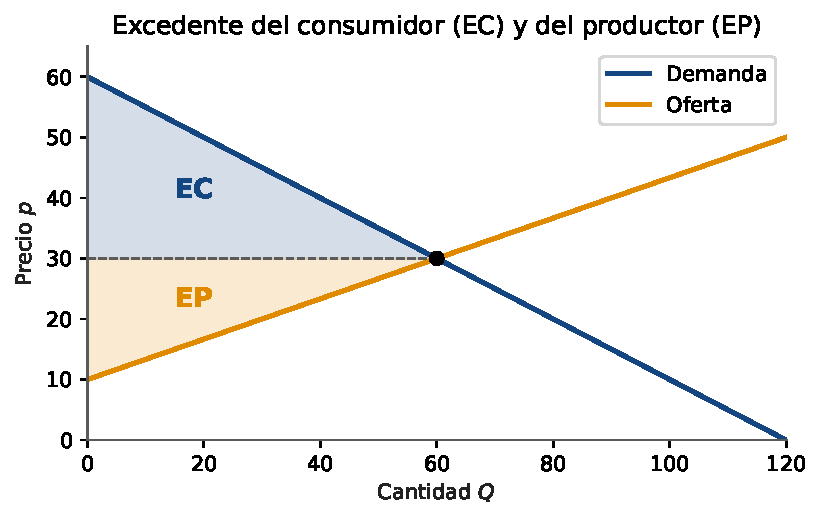
\includegraphics[width=0.72\linewidth]{figuras/excedentes}
\caption{El excedente del consumidor (EC) es el área entre la demanda y el precio; el del productor (EP), entre el precio y la oferta. Su suma es el bienestar total del mercado.}
\label{fig:excedentes}
\end{figure}

\begin{ideabox}
\textbf{Por qué importa.} Los excedentes son la forma en que la economía \emph{mide el bienestar}. Permiten evaluar políticas (un impuesto, un control de precios, una fusión) en términos de cuánto ganan o pierden consumidores y productores. Es el puente entre la microeconomía positiva («qué pasa») y la normativa («qué conviene»).
\end{ideabox}

\begin{labbox}
En el laboratorio, integrar es \texttt{sympy.integrate(f, (Q, a, b))}. El excedente del consumidor sale de integrar la demanda inversa menos el precio de equilibrio; el del productor, el precio menos la oferta inversa. Recordá la trampa: \texttt{sympy.integrate} no agrega la constante, así que para reconstruir el costo total hay que sumar el costo fijo a mano, tal como en la ecuación~\eqref{eq:costo_desde_cmg}.
\end{labbox}

\section{Síntesis del capítulo}

La integral acumula: reconstruye totales a partir de marginales y, sobre todo, mide los excedentes que cuantifican el bienestar de consumidores y productores. Con derivadas (medir el cambio) e integrales (acumularlo) ya tenemos todo el cálculo necesario para abordar el problema central de la empresa: optimizar.
